The impact of pileup effects on the performance of the CNN tagger is evaluated 
by considering events with a different number of reconstructed primary vertices ($N_\text{PV}$).
The test sample is divided into three bins: $N_\text{PV}<13$, $13<N_\text{PV}<20$ and $N_\text{PV}>20$.  
The distributions of the pixel intensities do vary with pileup, 
but the performance of the CNN tagger is found to be robust. 
This is demonstrated by Figure~\ref{fig:pileup}. 
% shows that the efficiencies for a specific working point vary with the pileup conditions (by a similar amount as jet width), but the overall discriminating performance is not significantly degraded (ROC curve is largely invariant).

\begin{figure}[tbp]
\begin{center}
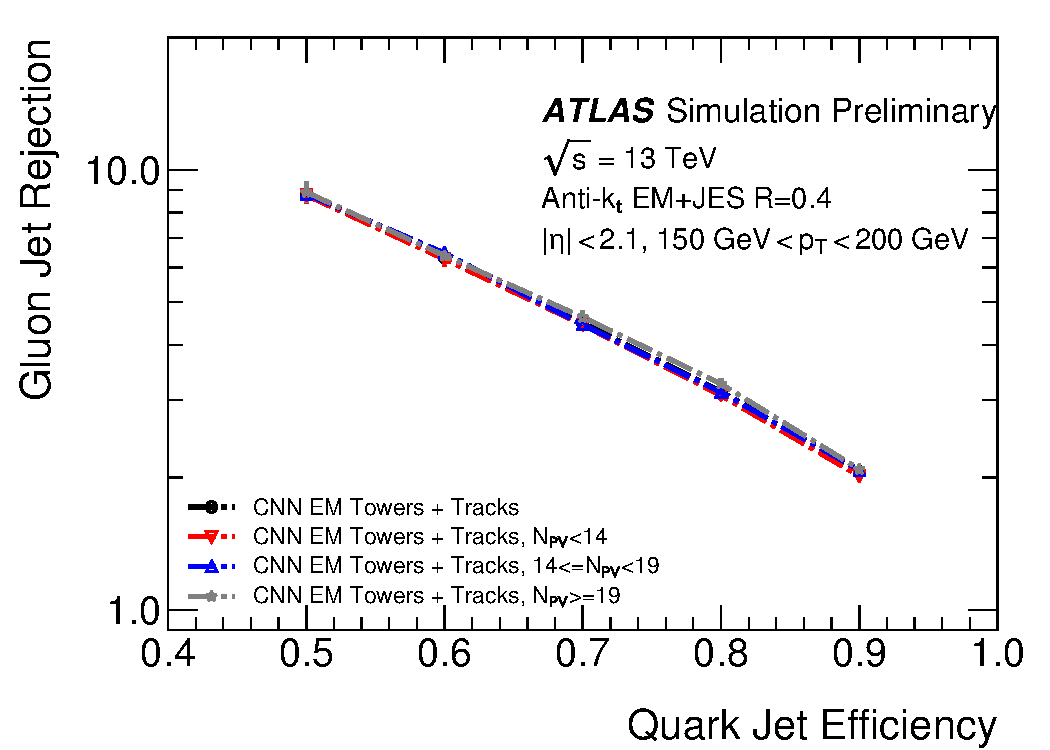
\includegraphics[width=0.5\textwidth]{figures/roc/ROC_pt150_200_NPV.pdf}
%\subfloat[][]{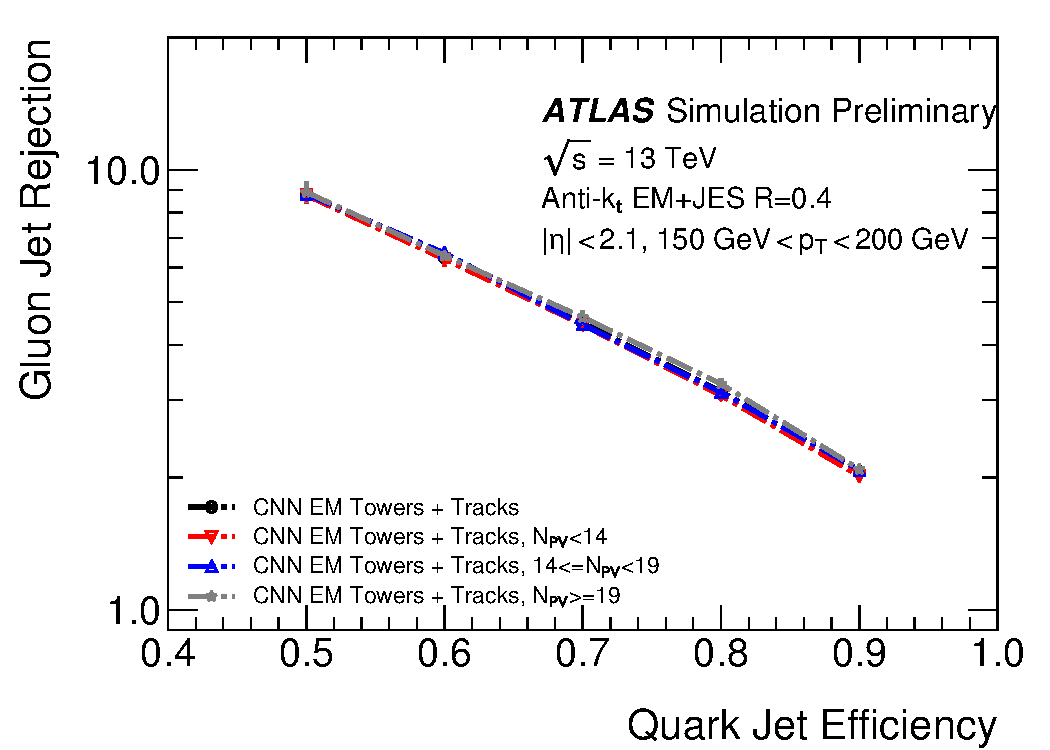
\includegraphics[width=0.5\textwidth]{figures/roc/ROC_pt150_200_NPV.pdf}\label{roc}}
%\subfloat[][]{\includegraphics[width=0.5\textwidth]{figures/roc/NPVEff.pdf}\label{eff}}
\caption{Gluon jet rejection as a function of the quark jet efficiency %\protect\subref{roc} 
evaluated at different pileup conditions, 
quantified by the number of reconstructed primary vertices ($N_\text{PV}$).}
%\protect\subref{eff} 
%Quark and gluon jet efficiency as a function of NPV for the CNN tagger.
%Jets are selected by requiring a minimum value of the CNN tagger, 
%where the threshold is chosen to give an overall 60\% quark jet efficiency.
%The efficiencies for jet width are shown for reference.}
\label{fig:pileup}
\end{center}
\end{figure}

Calorimeter-based discrimination is not only effected by in-time pileup (quantified by $N_\text{PV}$) but also by out-of-time pileup. 
Figure~\ref{fig:pileup2} compares the tagger performance in two different regimes of the average number of collisions per bunch crossing ($\mu$) regimes corresponding to the out-of-time pileup representative of LHC Run 2 conditions.

\begin{figure}[tbp]
\begin{center}
\subfloat[][]{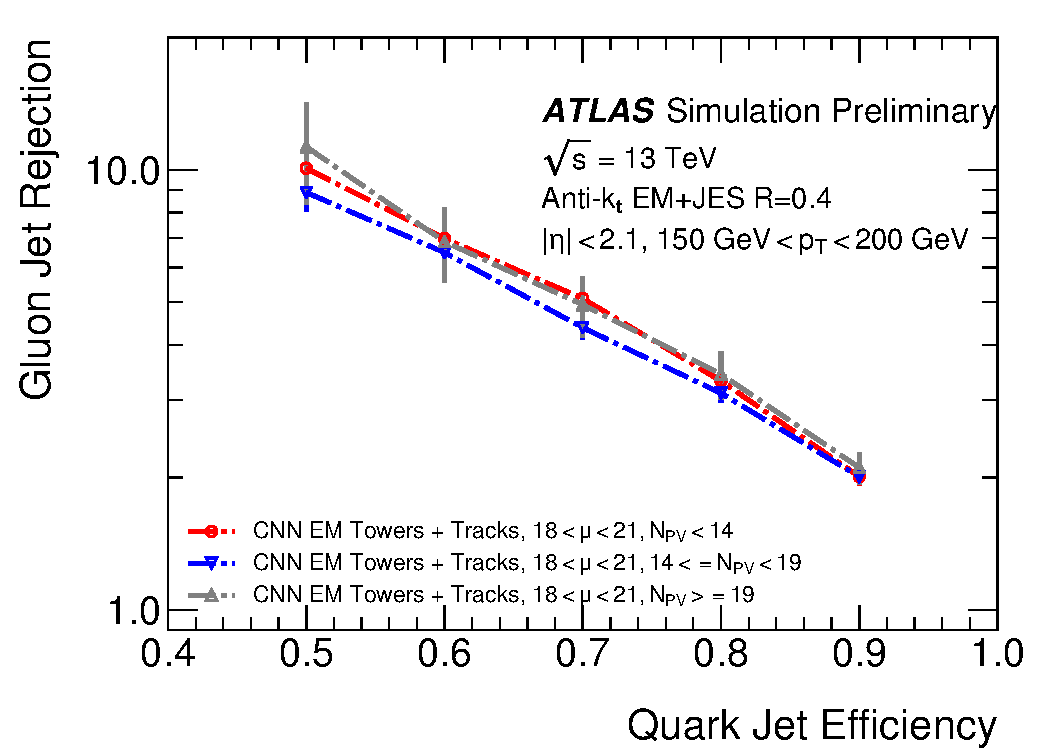
\includegraphics[width=0.5\textwidth]{figures/roc/ROC_pt150_200_mu18_21.pdf}\label{roc1}}
\subfloat[][]{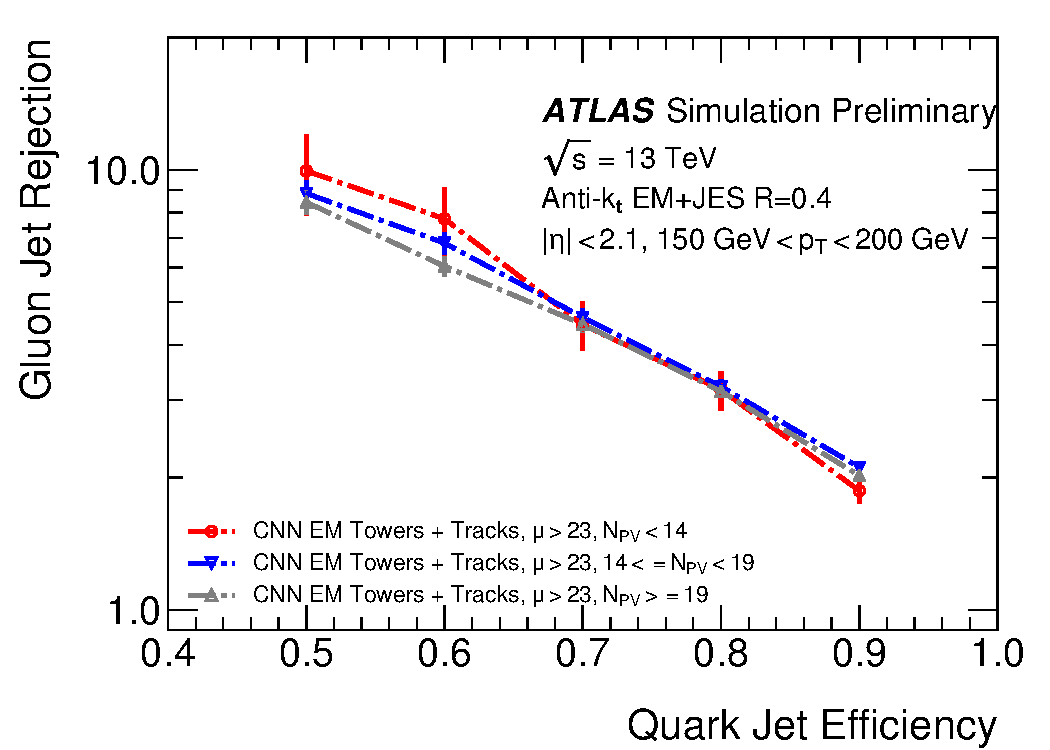
\includegraphics[width=0.5\textwidth]{figures/roc/ROC_pt150_200_mu23.pdf}\label{roc2}}
\caption{Gluon jet rejection as a function of the quark jet efficiency 
evaluated at different levels of $N_\text{PV}$ for \protect\subref{roc1} $18<\mu<23$ and \protect\subref{roc2}  $\mu > 23$.
The two $\mu$ bins where chosen to have roughly the same number of events.}
\label{fig:pileup2}
\end{center}
\end{figure}
